\subsection{2.3 Brazilian test}
\label{sec:brazilian_test}
\framecard{2.3 Brazilian test}
\begin{frame}{Set up}
	\bfc{\igwf{configuration_brazilian_test}{110mm}}{Set up [Credits: G. Puel]}{}
\end{frame}

% Set up
\begin{frame}{Set up}
\txb{120}{3}{12}{
	\begin{block}{Stress description}
		\begin{itemize}
			\item $\xv=r\ir\pdp{\theta}+z\iz,\quad \quad \pdp{r,\theta,z}\in \Omega_t=\left]0,\frac{D}{2}\right[\times\left]0,2\pi\right[\times\left]0,H\right[$
			\item $\stress\pxp=k\frac{\cos\theta_1}{r_1}\ir[1]\pdp{\theta_1}\otp\ir[1]\pdp{\theta_1} + k\frac{\cos\theta_2}{r_2}\ir[2]\pdp{\theta_2}\otp\ir[2]\pdp{\theta_2}-\frac{k}{D}\pdp{\ID-\iz\otp\iz}$
		\end{itemize}
	\begin{center}
		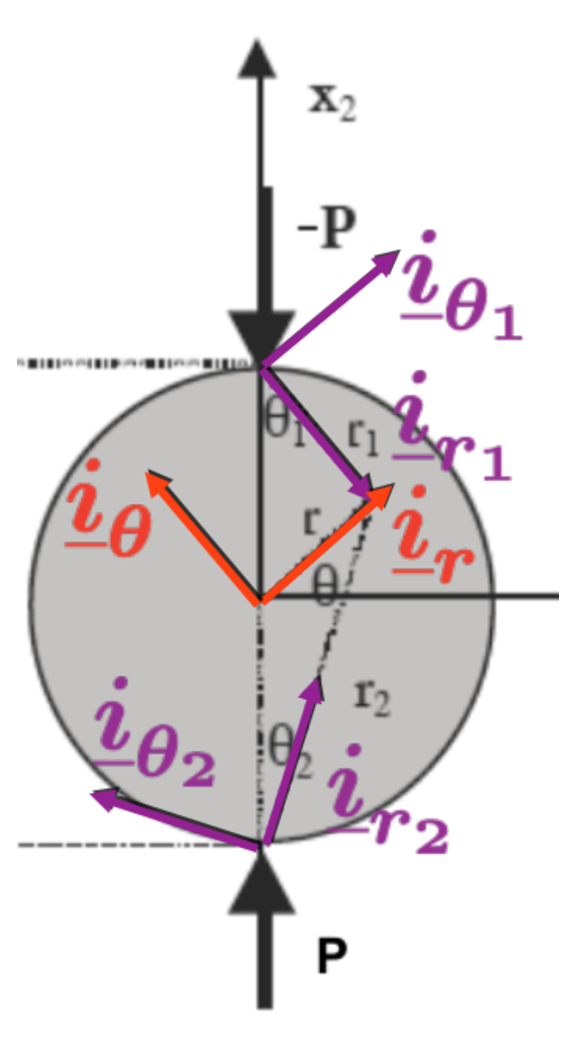
\includegraphics[width=30mm]{brazilian_test_1.eps}
	\end{center}

		\end{block}
}
\end{frame}

% Compute divergence stress
\begin{frame}{Check equilibrium}
	\txb{120}{3}{12}{
		\begin{exampleblock}{Question 1: $div_x\pdp{\stress\pxp}=0$?}
			\begin{itemize}
				\item $div_x\pdp{k\frac{\cos\theta}{r}\ir\pdp{\theta}\otp\ir\pdp{\theta}}=0$?
				\begin{enumerate}
					\item[$\square$] $\pard[][r]\pdp{k\frac{\cos\theta}{r}\ir\pdp{\theta}\otp\ir\pdp{\theta}}=-k\frac{\cos\theta}{r^2}\ir\pthp\otp\ir\pthp$
					\item[$\boxtimes$] $\pard[][\theta]\pdp{k\frac{\cos\theta}{r}\ir\pdp{\theta}\otp\ir\pdp{\theta}}=-k\frac{\sin\theta}{r^2}\ir\otp\ir+2k\frac{\cos\theta}{r}\ir\sotp\ith$
					\item[$\boxplus$] $\pard[][z]\pdp{k\frac{\cos\theta}{r}\ir\pdp{\theta}\otp\ir\pdp{\theta}}=0$
				\end{enumerate}
		
				$\to div_x\pdp{k\frac{\cos\theta}{r}\ir\pdp{\theta}\otp\ir\pdp{\theta}}=\square.\ir+\boxtimes.\frac{\ith}{r}+\boxplus.\iz=-k\frac{\cos\theta}{r^2}\ir+k\frac{\cos\theta}{r^2}\ir+0=0$\\
				{\scriptsize
				$$\hspace{-5mm} div_x\pdp{\stress\pxp}= div_x\pdp{k\frac{\cos\theta_1}{r_1}\ir[1]\pdp{\theta_1}\otp\ir[1]\pdp{\theta_1}}+div_x\pdp{k\frac{\cos\theta_2}{r_2}\ir[2]\pdp{\theta_2}\otp\ir[2]\pdp{\theta_2}}+$$\\$$+div_x\pdp{\frac{k}{D}\pdp{\ID-\iz\otp\iz}} =0$$
			}
			\end{itemize}	
		\end{exampleblock}
	}
\end{frame}

% Compute tractions on border
\begin{frame}{Boundary conditions}
	\txb{120}{3}{12}{
		\begin{exampleblock}{Question 2: $\stress.\nv\vert_{\partial\Omega_t}=0$?}
			\begin{enumerate}
				\item $\stress\vert_{\partial\Omega_t}=\stress\pdp{\frac{D}{2},\theta,z}$
				\item $\nv=\ir$
				\item on $\partial\Omega_t$: $\theta_2=\frac{\pi}{2}-\theta_1,\quad r_i=\frac{D}{2}\cos\theta_i (i=1,2),\quad \pscl{\ir[1]}{\ir[2]}$
				\item $\stress.\nv=\stress.\ir=k\sum_{i=1}^{2}\pdp{\frac{\cos\theta_i}{r_i}\pscl{\ir[i]}{\ir}\ir[i]}-\frac{k}{D}\ir$\\
				$\stress.\ir\vert_{\partial\Omega_t}=\frac{2k}{D}\sum_{i=1}^{2}\pdp{\frac{\cos\theta_i}{\cos\theta_i}\pscl{\ir[i]}{\ir}\ir[i]}-\frac{k}{D}\ir=0$
			\end{enumerate}

		\end{exampleblock}
	}
\end{frame}

% Numerical Stress field
\begin{frame}{Stress field}
		\begin{center}
	\ighf{brazilian_test_2}{60mm}
\end{center}
\end{frame}

% Vertical cut
\begin{frame}{Traction forces on horizontal cut}
	\txb{120}{3}{10}{
		\begin{exampleblock}{Question 3: Compute force $\Fv[][\text{UP}\to\text{DOWN}]$}
		{\scriptsize
			\begin{itemize}
				\item $\Fv[][\text{UP}\to\text{DOWN}]=\int_{\Sigma_{\text{hor}}} \stress\nv ds = \int_{\Sigma_{\text{hor}}} \stress\itwo ds$
				\item on $\Sigma_{\text{hor}}$: $r_1\cos\theta_1=r_2\cos\theta_2,\quad x_1\in\left]-\frac{D}{2},\frac{D}{2}\right[, x_1=r_1\sin\theta_1=r_2\sin\theta_2 (\theta_1=\theta_2=\alpha,r_1=r_2=\rho)$
				\item  on $\Sigma_{\text{hor}}$: $\pscl{\ir[1]}{\nv}=\pscl{\ir[1]}{\itwo}=\cos\alpha;\quad\pscl{\ir[2]}{\nv}=\pscl{\ir[2]}{\itwo}=-\cos\alpha$
				\item $\stress\vert_{\Sigma_{\text{hor}}}=\frac{kD}{2\rho^2}\cos\alpha\pdp{\ir[1]-\ir[2]}-\frac{k}{D}\itwo=\frac{kD}{\rho^2}\cos^2\alpha\itwo-\frac{k}{D}\itwo=\frac{kD^3}{4\pdp{\frac{D^2}{4}+x_1^2}^2}\itwo-\frac{k}{D}\itwo=\frac{k}{D}\pdp{\frac{1}{4\pdp{1+x^2}^2}-1}\itwo\Rightarrow\Fv[][\text{UP}\to\text{DOWN}]=\frac{k}{D}\pdp{\frac{1}{4}\pdp{\frac{x}{2\pdp{1+x^2}}+\frac{a\tan x}{2} }\Big\vert_{-\frac{D}{2}}^{+\frac{D}{2}}-D}\itwo=-P\itwo$\\
				$$k=-\frac{2P}{\pi}$$
			\end{itemize}
		}
		\end{exampleblock}
	\begin{center}
		\ighf{brazilian_test_3}{20mm}\ighf{brazilian_test_5}{20mm}
	\end{center}
	}
\end{frame}


% Horizontal cut
\begin{frame}{Traction forces on vertical cut}
	\txb{120}{3}{12}{
		\begin{exampleblock}{Question 3: Compute force $\Fv[][\text{RIGHT}\to\text{LEFT}]$}
			{\scriptsize
				\begin{itemize}
					\item $\Fv[][\text{RIGHT}\to\text{LEFT}]=\int_{\Sigma_{\text{ver}}} \stress\nv ds = \int_{\Sigma_{\text{ver}}} \stress\ione ds$
					\item on $\Sigma_{\text{ver}}$: $\theta_1=\theta_2=0, \quad x_2\in\left]-\frac{D}{2},\frac{D}{2}\right[,x_2=D-r_1=r_2-\frac{D}{2}\quad \ir[1]=\itwo=-\ir[2]$
					\item  on $\Sigma_{\text{ver}}$: $\frac{\cos\theta_1}{r_1}\ir[1]\otp\ir[1]=\frac{1}{r_1}\ir[1]\otp\ir[1]; \frac{\cos\theta_2}{r_2}\ir[2]\otp\ir[2]=\frac{1}{r_2}\ir[1]\otp\ir[1]$
					\item $\stress.\ione\vert_{\Sigma_{\text{ver}}}=k\frac{r_1+r_2}{r_1 r_2}\itwo\otp\itwo.\ione-\frac{k}{D}\ione=-\frac{k}{D}\ione>0 \quad \text{TRACTION!}$
				\end{itemize}
			}
		\end{exampleblock}
		\begin{center}
			\ighf{brazilian_test_4}{25mm}\ighf{brazilian_test_6}{25mm}
		\end{center}
	}
\end{frame}

